\chapter{Computer Experiments} \label{ch:computer_experiments}
How to deal with big datasets that will easily eat up you memory? ``Big data'' involve processing large amounts of data that does not fit into memory. Processing ginormous amounts of data require expert knowledge about distributed systems and analysing for system bottlenecks. This section describes the computational experiments conducted in this thesis, and related issues encountered during the software development. 

The downloaded size of \acrshort{ecc} is 17Gb, stored in \acrshort{netcdf}-files. 
In comparison to related works by \citeauthor{precip_nowcasting} (\citeyear{precip_nowcasting}) and \citeauthor{SunAirLSTM} (\citeyear{SunAirLSTM}), using datasets of size X and Y respectively, this is a lot more.
%In comparison to ImageNet 2012 \textbf{source link to tensorflow docs} with downloading size is 144.02 GiB it is small. 
%However its impossible to work on the full dataset from the authors Lenovo E31 laptop. 
Conducting experiments on large datasets require external computational resources. %Storing is more important since the raw data used in the compilation of the dataset amount to several hundreds of Gb.

The results from the experiments conducted based on the setup and configuration. %presented in Section \ref{sec:hyperparam_tuning}. 
Finally, each model is evaluated on unseen portion of the dataset. Although theoretically fascinating it remains to see if \acrshort{convlstm} provide a clear practical advantage over the autoregressive models.

\section{Hardware}
\textit{The best choice of collective implementation depends upon the number and kind of GPUs, and the network interconnect in the cluster.} Efficient pipelines and traning procedyres. This project had access to a DGX-2 system consisting of 16 NVIDIA Tesla V100 GPUs, each of 32Gb local memory and 1.5Tb shared memory. The resources is availble through the \acrfull{ex3} project hosted at Simula. This project is allowed to use 1 GPU and X part of the memory. 

%\textit{NVIDIA V100 GPU -- The eX3 infrastructure includes a DGX-2 system consisting of 16 NVIDIA Tesla V100 GPUs, allowing simultaneous communication between all eight GPU pairs at 300 GBps through the 12 integrated NVSwitches. This gives a theoretical system-wide system bi-directional  bandwidth of 2.4 TBps. All GPUs have 32 GB of local memory (total of 512 GB) and share a 1.5 TB main memory. The total system has 81,920 CUDA cores, and 10,240 Tensor cores delivering 2 Petaflops of tensor performance. The peak performance in double precision is 125 Teraflops.}

\textit{This system designed for billion-way concurrency also represents a major challenge with many features: How to program such computers? How to port existing code, and how to reach a satisfactory level of reliability and efficiency while maintaining an acceptable energy footprint? How do you even debug software running on such a beast? }

%\textit{The exponentially increasing need for computing power in science and society at large has fueled the quest for developing exascale computers capable of performing a billion billion (10\textsuperscript{18}) floating-point operations per second. This upcoming generation of high performance computing (HPC) will rely on an intricate interplay between thousands of sophisticated processing nodes, each with a large number of cores, deep memory hierarchies and equipped with accelerators, organized in complex communication topologies. Heterogeneity is expected on all hardware levels, such as the nodes may also include processors that are tailored for certain types of algorithms, for instance graph-oriented methods for machine learning. While there is no fixed blueprint for exascale computers, the aggregated level of complexity in a strongly heterogeneous system designed for billion-way concurrency also represents a major challenge with many features: How to program such computers? How to port existing code, and how to reach a satisfactory level of reliability and efficiency while maintaining an acceptable energy footprint? How do you even debug software running on such a beast? While competing technologies in hardware, middleware, and software are being driven by major research projects in the United States, China, Japan and the EU, it is essential for Norwegian HPC research groups to keep pace with the frontier research.}

\textit{The eX3 infrastructure will not be an exascale computer by itself, but it will be a carefully curated ecosystem of technology components that will be crucial for embracing exascale computing. It will allow HPC researchers throughout Norway and their collaborators to experiment hands-on with emerging HPC technologies – hardware as well as software.}

In this section \cite{ex3docs} and \cite{ex3homepage}.

\begin{table}[ht]
    \centering
    \begin{tabular}{c|c}
        Device &  Type  \\
        GPU & Tesla V100-SXM3-32GB 
    \end{tabular}
    \caption{Hardware specifications for our testing environment on eX\textsuperscript{3}. Operativ system er Ubuntu?}
    \label{tab:hardware_ex3}
\end{table}

Working on this cluster requires you to move your files for fst access, create a virtual enviornment to use, relocate you code (here donw using brances on github) and schedule tasks on a GPU using a slurm scheduler. 
\textbf{Vær forsiktig med å si at du ike trenger å parallellsisere, det er litt mystisk når du leser på egen errormeldingene.}

Its desirable to have a fast access to the data. On ex3 this is done by a Remote Direct Memory Access (RDMA) over Infiniband.

\section{Software -- need to sort content}
The tensorflow keras API simplifies many aspects of building and executing machine learning models. Its implementation and distribution system aware. 

Distributed programming involves splitting the data into many tasks. These tasks are then executed in parallel by workers also known as threads. Parallel programming is necessary to take advantage of all the cores on a cluster to accelerate computational science. 

Complex computations will cause memory growth, dependant on how many intermediate computations it needs to store.

For fast debugging, the programs are implemented using dummy data or a subset of the dataset. Expanding the data amount to the entire dataset can require additional adjustments. For instance, the threads run on the problem of linear regression deadlocks upon the extraction of large amount of data. This is a precautionary measure to avoid overloading the system(\textbf{or server or cluster}).
%, which is a good thing. 
However, working on dummy data or smaller portion of the dataset might misleading with regard to how close you actually are to a solution. The solution here is to extract the data before the thread is started.

%Implementing a pixel wise regression seems like a straight forward task. And it is, as long as you can keep track of memory requirements, and extract the data before it is sent into the thread.

%Hardware problems; quick data flow (dependant on the disk it is stored on), and enough memory.
%The choice of software implementation can create a 
File structure is also important, ideally data should be stored in a fashion that you don't load to much into memory. For the \acrshort{convlstm} case that would be a grid of time series, as done in this project, but for the pixelwise regression case it could be beneficially too store one pixel at a time. Storing the data in this manner will again force you to request data from the storage space more frequent, but it could ease the paralization of the program. However, there is no guarantees this will give you more bang for the buck. 


\section{Framework - Model Setup}
\textbf{Manuel tuning since the computational resources easily get exhausted depending on the architecture}
\textbf{The architecture is dependant on the problem, but also the memory resources.}

The following sections contain the configurations of the models compiled for this thesis along with descriptions of hyperparameters. Recall that a hyperparameter is a parameter set before the training starts, as mentioned in Section X. A model is compiled based on a choice of hyperparameters. In the search for the best model configuration, different combinations of hyperparameters are tested. This is done manually. It is possible since \acrshort{ar}-models have a small search space.  The \acrshort{convlstm} models have a large search space. As a starting point a set of architectures used by \citeauthor{SunAirLSTM} (\citeyear{SunAirLSTM}) on a similar problem, air quality forecasting problem was executed. \citepaper{chollet2015kerastuner} provide suitable software for the automatic hyperparameter tuning. 

\textbf{Man kjører eksperimenter på mange modeller ved å bruke traning og validations dataset. The choice of model is based on this data basis and then it performance is tested on the test dataset. }
Inherited from the problem the \acrshort{ar}-models dataset is split into two portions, training and test. This is sufficient, since there exist an analytical solution to this problem, as mentioned in Section \ref{sec:ARmodels}. For the \acrshort{convlstm} there is no analytical solution, there is a numerical solution, this introduce the need for a validation dataset. Both model are tested on 2014 to 2018. For \acrshort{ar}-models this is trained on 2004 to 2013 and the \acrshort{convlstm} trained on  2004 to 2011 and validated on  2012 to 2013. The test period was chosen based on the assumption that the latest period is most representabel for the climate in the near future.

Other minor differences for the datasets prepared for the \acrshort{ar} and the \acrshort{convlstm}-models. The order of the \acrshort{ar}-model determine the length of the training sequence. All samples with gaps in the requested sequence is disregarded causing a reduction in the data basis for a particular model. For the \acrshort{convlstm} these gaps are filled with a out-of-sample value, $c=1.5$.

\subsection{Autoregressive models}
%\textbf{Move first two paragraphs to discussion..?}
The python package ``sciclouds'' provide a self implemented version of \acrshort{ar}-models, using the analytical solution to the least squares problem derived in Section \ref{sec:ARmodels}. This has major improvement possibilities. 

A set of models are compiled by varying components like scaling the predictors, transforming the target, the inclusion of intercept, order of the models and environmental variables. One AR-model is the combination of 13041 individual regression models. Time consuming task because of the high number of matrix inversions. A double for loop over this takes to long and \textbf{mention the version of paralelization used on this problem}.

\subsubsection{Feature Scaling} \label{sec:scaling_predictors}
%Feature standardization makes the values of each feature in the data have zero-mean 

Feature scaling is used to standardise or scale the predictor variables. By subtracting the mean and dividing by the variance, the distribution is reshaped to a standard normal distribution with zero mean and unit variance. Data transformation can be beneficially in an attempt to achieve numerical stability. When applied the predictors is transformed according to the following Equation \ref{eq:scaling_data}. The feature scaling is applied after the partition into training and test dataset, the mean and standard deviation is computed based on the training set. If it was done based on the entire dataset, the trained model would have sneak peaked at the test data.
\begin{equation} \label{eq:scaling_data}
    \mathbf{x} = \frac{\mathbf{x} - \bar{\mathbf{x}}}{\sigma_{\mathbf{x}}}
\end{equation}
where $\bar{\mathbf{x}}$ is the average and $\sigma$ is the standard deviation.
The mean and standard deviation is applied to the test dataset. This is necessary to since the model is now trained to find relations in transformed data, the raw data is out-of-sample.

\subsubsection{Transforming target} \label{sec:transforming_target}
A trick in avioding prediction unphysical values is fitting agains a transformed target. Since the target, \acrfull{cfc}, is within the ranges of 0 and 1. Can be transformed to values from the entire real axis $(-\infty, \infty)$. The inverse transformation truncates the values in the range or [0, 1], alleviation predictions of out-of-sample values. A function suitable for this task is the sigmoid function, shown in figure \ref{fig:activation_func_plus}. 
\begin{figure}
    \centering
    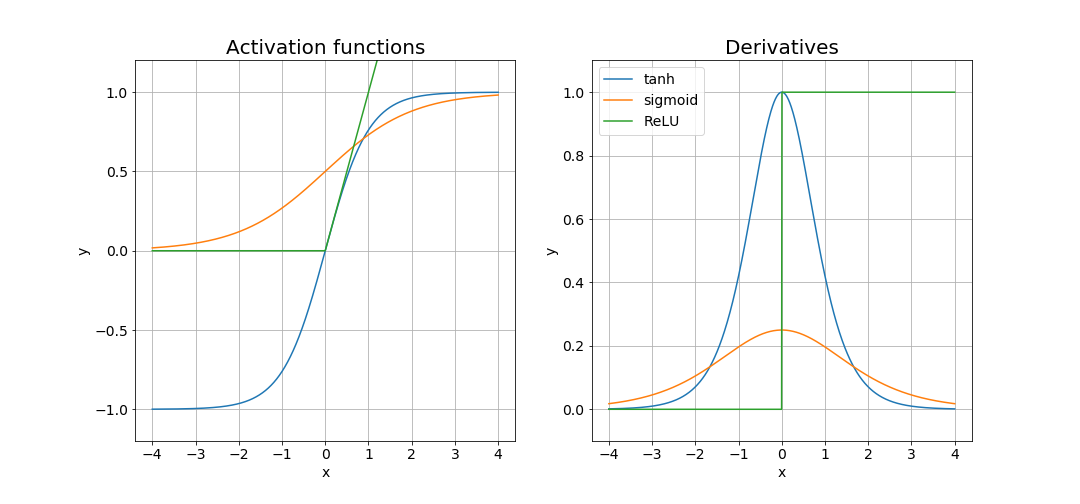
\includegraphics[scale=0.45]{Chapter3_Method/figs/activation_functions_and_derivatives.png}
    \caption{Activation functions used }
    \label{fig:activation_func_plus}
\end{figure}

\subsubsection{Order and Environmental variables}
The dataset for a particular model is a combination of the order, the number of time steps of previous cloud cover includes as predictors and the inclusion of environmental variables, temperature, surface pressure, specific and relative humidity. All model is trained either on the full set of environmental variables or none of them.

\subsubsection{Experimental setup AR-models}
Table \ref{tab:ar_model_config} shows a summary of the \acrshort{ar}-models included in this thesis. 

\begin{table}[h]
    \centering
    \resizebox{\textwidth}{!}{%
    \begin{tabular}{ccccc}
    \cline{2-5}
     & \textbf{Scaling predictors} & \textbf{Transforming target} & \textbf{Order} & \textbf{Enviornmental variables} \\ \hline
    \multicolumn{1}{c}{\textbf{Model 1}} & \checked & $\times$  & 1 & $\times$ \\ \hline
    \multicolumn{1}{c}{\textbf{Model 2}} & \checked & $\times$  & 0 & \checked   \\ \hline
    \multicolumn{1}{c}{\textbf{Model 3}} & \checked & $\times$  & 1 & \checked  \\ \hline
    \multicolumn{1}{c}{\textbf{Model 4}} & \checked & $\times$  & 2 & \checked  \\ \hline
    \multicolumn{1}{c}{\textbf{Model 5}} & \checked & $\times$  & 3 & \checked  \\ \hline
    \multicolumn{1}{c}{\textbf{Model 6}} & \checked & $\times$  & 4 & \checked  \\ \hline
    \end{tabular}%
    }
    \caption{Configuration of \acrshort{ar}-models. $\times$ denoted not applied, \checked denotes applied \textbf{add bias??} Gi modellen navn basert på configurasjonen $AR_{STEx}$ where x is the order.}
    \label{tab:ar_model_config}
\end{table}

\subsection{Convolutional LSTM}
% Endrer på arkitekturen - denne bruker -train - validation - test, en hvis prosentandel a
Citation BatchNormalization \cite{ioffe2015batch}. 
A lot of architectural decisions can cause (batch size, sequence length, number filterers and number layer) can cause the \acrshort{gpu} to run out of memory. Future work speed up the \acrshort{ar}-model computations of self implemented modules for computations using  a C or C++ backend.

Tensorflow har pakker for å ha prosessert data i cache. For å unngå at det må prosesseres for hver epoch. 



The formulation of the Air quality forecasting problem presented by  \citeauthor{SunAirLSTM} is similar to the formulation of the cloud fractional cover prediction problem presented in this project. The machine learning experimental setup is adopted from the paper \citepaper{SunAirLSTM}. 


\section{Results}
Recall that all models are trained on X and tested on Y. The autoregressive model is optimized to get the cloud cover at a certain time, by feeding the model with the result from the previos predictions one can generate sequences with the AR-model. For the convolutional model, two seperate models need to be trained? Det stemmer vell ikke man kan vell bruke en modell som er trent på å return sequence (True) til å bare returne den første? \textbf{Litt usikker på struktur på trening og test data her.}
\subsection{Predicting next timestep}
Some text ....

\subsection{Predicting next 24 hours (or another sequence)}
Some text ....
input-to-state (input to first layer) and state-to-state transition (internal layer to internal layer)

\subsection{Autoregressive models}

%%%% TARGET PREDICITON HORIZONTAL
\begin{figure}[ht]
    \centering
    \includegraphics{python_figs/target_prediction_plot_horizonal.pdf}
    \caption{Comparison target and predicted cloud fractional cover.}
    \label{fig:target_predict_horizontal}
\end{figure}

%%%% TARGET PREDICITON HORIZONTAL
\begin{figure}[ht]
    \centering
    \includegraphics{python_figs/target_prediction_plot_vertical.pdf}
    \caption{Comparison target and predicted vertical cloud fractional cover.}
    \label{fig:target_predict_vertical}
\end{figure}

%%%% TARGET PREDICITON ERA5
\begin{figure}[ht]
    \centering
    \includegraphics{python_figs/target_prediction_era5_plot_horizonal.pdf}
    \caption{Comparison target, predicted and era5 horizontal cloud fractional cover.}
    \label{fig:target_predict_era5_vertical}
\end{figure}

\subsection{Convolutional Long Short-Term Memory network}
Either summaries the findings into one table 


\section{Experiments}



The statistical properties are slightly different for the different test sets.  

Short sequnece length to reduce the computational com-
plexity of experiments. 

No efforts have been made to assess the impact of the artefact on the performace.

One variable was not found to increase the performance.


data sets can be reduced without significant loss of information

A drawback of this study was not to account for correlations between radiomics features and the ROI, but such corrections were
not performed in this thesis.

Land ocean mask study statistics of subgroups.


\section{Practical implications - OUTDATED} \label{sec:practical_implications}
It is necessary to have a understanding of the needs of the end product before conducting large machine learning projects. Answering questions like: What will it be used for and how can it be implemented in useful way?

A major downside of the data driven learning approach is the rigid resolution. A trained model can only be used on similar problems, with the same spatiotemporal resolution. For applications like climate models, output comes in a wide range of different resolutions. Before implementing the finished product in a new model of a different resolution, it would need to be retrained on the resolution of the climate model under development. This process involves both remapping of the dataset and retraining the model at the correct resolution. This is a time consuming process involving finding a new set of hyperparameters suitable for the new resolution. % It essentially means starting over.

Once trained on global climate datasets, machine learning models provide fast results even for complex parameterization which is what makes them suitable for the application of climate modelling. Most machine learning packages are developed using Python. \acrfull{esm} are implemented in python. Methods for including the trained parameterizations need to be developed.
 
\subsection{Any implications based on the results presented in this chapter.}